\section*{Источники и решения}

\subsubsection*{Падение Элиса}

Насколько мне известно, первая публикация этой замечательной головоломки состоялась в веб-колонке «Math Fun Facts» Фрэнсиса Су из Колледжа Харви Мадда;
Фрэнсис припоминает, что услышал её в Европе от некого Феликса Варди, кого он не смог найти.
После этого головоломка появилась в журнале Emissary \cite[Весна/Осень 2003]{berlekamp-buhle}.

Дэн Амир, бывший ректор Тель-Авивского университета, увидел головоломку в Emissary и предложил её тель-авивскому математику Ноге Алону, который принёс её в Принстонский Институт перспективных исследований;
я же услышал её от Ави Вигдерсона из этого института в конце 2003 года.

Ключ к этой и последующим головоломкам в том, что если бы муравьи были взаимозаменяемы, то было бы без разницы, проходят они сквозь друг друга или разворачиваются при встрече.
Тогда каждый муравей просто идет прямо и должен упасть в течение 100 секунд.
Поскольку через 100 секунд все муравьи упали, то упал и Элис.

Если хочется избежать анонимности муравьев, то можно думать, что каждый из них несёт флажок.
При встрече они обмениваются флажками и разворачиваются.
Таким образом, каждый муравей всегда несёт один флажок, и флажки проходят мимо друг друга.
Если со стержня исчезли все флажки, то исчезли и муравьи.

Если начать с муравья, стоящего лицом на восток на западном конце шеста, то легко сделать так, чтоб Элис через 100 секунд понёс его флажок к восточному конецу.
Поэтому 100 секунд ожидания необходимы и достаточны.

\subsubsection*{Элис на окружности}

Как и раньше, будем думать, что муравьи несут по флажку, и обмениваются ими при встрече.
Тогда каждый флажок проходит полный круг за заданный период времени, заканчивая там, где начал.
При этом циклический порядок муравьёв не меняется, и значит (в большинстве случаев) произошёл циклический сдвиг.
То есть каждый муравей сдвинулся на определённое число позиций, скажем $k$, по часовой стрелке.
В частности, если Элис вернулся на своё место, то вернулись и все остальные.

Заметим, что если изначально $m$ муравьев смотрят по часовой стрелке, то в любой момент времени $m$ муравьев идут по часовой стрелке, а $24 - m$ против.
Ведь при каждом столкновении муравей, движущийся по часовой стрелке, становится движущимся против часовой стрелки, и наоборот;
про это можно думать как сохранение момента импульса!
В любом случае, за время всего эксперимента один муравей сдвинуться в среднем на $100(2m - 24)/24$ сантиметра по часовой стрелке.
Значит, каждый вернётся на своё место тогда и только тогда, когда $2m - 24$ кратно $24$; то есть, если $m = 0$, $24$ или $12$.

Первые два варианта (когда все муравьи изначально смотрят в одном направлении) имеют незначительную вероятность, но вклад последнего составляют внушительные $16,1180377\%$.

Чтобы быть совсем точными, у нас есть $2^{24}=16\,777\,216$ вариантов выбрать направления из которых  $\binom{24}0+\binom{24}{12}+\binom{24}{24}=1+1+2\,704\,156$ возвращают Элисa на место.
Это дает вероятность $2\,704\,158/16\,777\,216 \z\sim 0{,}161180377$.

\subsubsection*{Какой конец?}

Заметим, что число муравьев, падающих с восточного конца стержня, такое же, как число муравьев, смотрящих на восток в начале.
Действительно, число муравьев, смотрящих на восток, никогда не меняется.???
(Также вы можете думать об упавших со стержня флагах).
В любом случае, если $k$ муравьев выпадают с восточного конца, то именно это делают $k$ самых восточных муравьев, поскольку сохраняется порядок муравьёв на стержне.

Воспользовавшись симметрией, можно предположить, что в начале Элис смотрит на восток.
Как мы уже знаем, он упадёт с восточного конца тогда, когда число муравьев, смотрящих на восток, составляет как минимум $13$. Это означает, что $12$ или более из оставшихся $24$ смотрят на восток.
Вероятность того, что $13$ или более из $24$ муравьев смотрят на восток, такая же, как вероятность того, что $11$ или менее смотрят на восток, поэтому вероятность события, которое нас интересует, равна половинке плюс половине вероятности того, что ровно 12 из
24 муравьев смотрят на восток.

Последняя составляет $\binom{24}{12}/2^{24}$, что дает $0{,}161180258$;
следовательно, ответ составляет $0{,}580590129\dots$ --- немного больше чем 58\%.

\subsubsection*{Кто последний?}

Можно предположить (снова используя симметрию), что Элис падает с восточного конца,
а значит и $12$ муравьев к востоку от него делают то же самое.
Если он падает последним, то 12 муравьев к западу от Элис упадут с западного конца.
То есть изначально 12 флажков, а значит, 12 муравьев, смотрят на запад. Это происходит с вероятностью $\binom{25}{12}/2^{24}$, то есть примерно в $31\%$ случаев.

Однако и в этом случае Элис не обязательно падает последним; примерно в половине случаев эта честь достаётся его западному соседу.
Таким образом, интересующая нас вероятность будет около $15.5\%$.

Но не стоит довольствоваться приближением, когде можно найти точный ответ.
Время, которое каждый флаг обречен провести на стержне, независимо и равномерно случайно между $0$ и $100$ секундами.
Таким образом, вероятность того, что самый долгоживущий флажок это один из 13 восточно-направленных флажков, составляет $13/25$.
Отсюда следует, что правильное значение составляет $13/25 \z\times\binom{25}{12}/2^{24}$, а это равно уже знакомому нам $\binom{24}{12}/2^{24}\sim 0{,}161180258$.

\subsubsection*{Число столкновений}

Каждый флажок сойдётся со всеми флажками перед ним направленных к нему;
для флажка в середине, это в среднем $6$ из $12$.
Таким образом, средний флаг сталкивается с шестью другими; следовательно, в среднем происходит $25 \times 6 = 150$ столкновений.
При этом каждое столкновение считается дважды, поэтому ответ составляет $75$.

Альтернативный и немного более строгий способ вычисления:
Какова вероятность того, что два флага столнутся?
Независимо от их местоположения, это происходит только если они смотрят друг на друга, таким образом, с вероятностью $\tfrac14$.
По линейности матожидания, число столкновений равно $\binom{25}2 \times \tfrac14 = 25 \times 24 /8 = 75$.

Максимальное число столкновений достигается, если все муравьи направлены к Элис (центральному муравью), в котором случае все $13$ флагов, смотрящих на Элис, сталкиваются с $12$ флагами, смотрящими в другую сторону, всего $12 \times 13 = 156$ столкновений.

Наименьшее возможное число столкновений, конечно, равно нулю, но это происходит с вероятностью только $26/225 \sim 0{,}000000774860382$.


\subsubsection*{Помятость Элиса}

Легко подсчитать столкновения флажка Элиса.
Пусть Элис изначально смотрит на восток, в среднем будет $6$ (из $12$) флагов перед Элисом, смотрят на запад.
Следовательно, в среднем  флажок Элиса столкнётся с шестью другими флагажками.

Но Элис не всегда несет свой исходный флаг, и ожидается, что у Элиса будет гораздо больше, чем шесть столкновений в среднем.
Почему?
Потому что в среднем у муравья шесть столкновений ($75 \times 2/25$), а Элис, стоя посредине, должен сталкиваться чаще.

Теперь, любой данный муравей сталкивается только со своими двумя соседями, и чередует их (поскольку его направление чередуется между столкновениями).
Последнее столкновение муравья будет с его западным соседом, если он в конечном итоге свалится с восточного конца, и с его восточным соседом, если он свалится с западного конца.

Давайте предположим, что изначально $k$ муравьев смотрят на запад.
Поскольку их флаги идут с западного конца стержня, $k$ муравьев на западе в конечном итоге сваливаются с западного конца.
Каждый муравей, который изначально смотрел на запад, имеет одинаковое число столкновений с каждой стороны;
те, кто смотрел на восток, имеют на одно столкновение больше на восточной стороне.
Таким образом, число столкновений между муравьем  номер $j$ (считая с запада) и муравьем 
$j+1$ равно числу муравьев, смотрящих на восток, среди муравьев от $1$ до $j$ --- при условии, что $<j<k$.

В силу симметрии можно предположить, что $k$ находится между $13$ и $25$ (то есть Элис сваливается с западного конца).
Тогда число столкновений между Элис и его западным соседом точно равно числу муравьев, смотрящих на восток, к западу от Элис; обозначим это число как $x$.
Общее число столкновений, испытываемых Элис, затем будет равно $2x$ или $2x+1$, в зависимости от того, смотрела ли она сама на запад или на восток в начале.

Априори математическое ожидание $\mathbb{E}[x]$ для $x$ равно $6$, так как западнее Элис находится $12$ муравьев, каждый из которых может смотреть в любом направлении.
Однако мы только что предположили (чорт!), что больше половины муравьев смотрят на запад.
Обратите внимание, что, поскольку ожидаемое число муравьев, смотрящих на восток, к востоку от Элис также равно $\mathbb{E}[x]$, число $2\mathbb{E}[x+1]$, которое мы ищем, является именно общим ожидаемым числом муравьев, смотрящих на восток, учитывая, что они в меньшинстве.

Предположим, что муравьи были распределены по направлениям в алфавитном порядке, а последним был муравей Зельда.
Существует...способа сделать такое распределение, чтобы получить большинство западных направлений;
из них ... приведут к $12$ муравьям, смотрящим на восток, среди первых $12$.
В этих случаях Зельда вынуждена смотреть на запад;
в остальных случаях она с равной вероятностью смотрит на запад или на восток. Следовательно, вероятность того, что она смотрит на восток, составляет 
$0{,}419409871$

Поскольку вероятность того, что Зельда смотрит на восток, не отличается от вероятности любого другого муравья, мы можем умножить это на $25$, чтобы получить ожидаемое число муравьев, смотрящих на восток, примерно $10{,}4852468$.
Именно это и является средним числом столкновений, которые переживает Элис.

\subsubsection*{Страховой рейтинг Элиса}

Предположим, что самые западные $k$ муравьев падают с западного конца,
а остальные с восточного.
Мы уже видели в предыдущем решении, что если $c_i$ --- число столкновений между муравьём $i$ (считая с западного конца) и муравьём $i + 1$, то $c_i$ остается тем же или увеличивается на $1$ до $i = k$; после этого остается тем же или уменьшается на $1$.
В частности, $c_i=c_{i-1}$ ровно тогда, когда муравей $i$ смотрит (изначально) в том we направлении, с которого on упадёт.

Число столкновений, переживаемых муравьем $i$, равно $c_{i-1}+c_{i}$. Значит, чтобы Элис выиграл в игре столкновений, нужно, чтобы $c_{11}+c_{12}<c_{12}+c_{13}>c_{13}+c_{14}$, а это означает, что  $c_{11}<c_{13}$ и $c_{12}>c_{14}$.
Это может произойти только если $c_{11}<c_{12}=c_{13}>c_{14}$, а значит что $k = 12$ или $13$, что Элис смотрит в том направлении, с которого падает,
и что оба его соседа смотрят в противоположные стороны от тех концов, с которых они падают.
Похоже, что вероятность 
\[(\binom{25}{12}+\binom{25}{12})/2^{25}\cdot (\tfrac12)^3\sim 3.87452543\%,\]
однако события не совсем независимы.

Предположим, что Элис смотрит на восток, его восточный сосед --- Эд, а западный сосед --- Уилл.
Затем Эд, как и Элис, будет падать с восточного конца и, следовательно, изначально должен был смотреть на запад (вероятность $1/2$).
Уилл будет одним из $12$ муравьев, падающих с западного конца и, следовательно, изначально смотрел на восток (вероятность $1/2$).
Из оставшиеся 22 муравьёв половина должна смотреть на запад, а половина на восток (вероятность $\binom{22}{11}/2$), поэтому точный ответ составляет 
\[(\tfrac12)^2\cdot\binom{22}{11}/2^{25}\sim 4{,}20470238\%.\]

\subsubsection*{Насморк}

Эта головоломка чисто комбинаторная, как и многие другие головоломки про Элиса.
В частности, хоть может показаться иначе, она никак не связана с длиной стержня.
Может показаться, что более короткий стержень может позволить некоторым муравьям выбраться с него до того, как они успеют заразиться, но как только муравей направляется к концу и перед ним нет других муравьев, его дни столкновений заканчиваются.

Вероятно, самый простой способ сделать необходимый расчет --- это представить, что заражаются не муравьи, а флаги. Мы можем предположить, что Элис смотрит на восток; тогда все флаги, направленные на запад впереди нее, пересекают ее флаг и заражаются, в то время как флаги, направленные на восток впереди нее, остаются не зараженными.
Тем временем флаги, направленные на запад, после пересечения с флагом Элис, заражают все флаги, направленные на восток позади Элис, в то время как флаги, направленные на запад позади Элис, уходят.

Поскольку в среднем впереди Элис находится 6 флагов, направленных на запад, и 6 флагов, направленных на восток, показалось, что это дает в среднем 13 зараженных флагов (включая флаг Элис) и, таким образом, 13 зараженных муравьев.

Однако есть небольшая ошибка: если впереди Элис нет муравьев, смотрящих на запад, тогда нет флага, чтобы пересечь флаг Элис и заразить флаги, направленные на восток, позади нее. Это происходит с вероятностью $1/2^{12}$ и уменьшает ожидаемое число зараженных с $7$ (Элис плюс в среднем 6 флагов, направленных на восток, позади нее) до 1 (только Элис) в этом случае.
Таким образом, правильный ответ не $13$, а $13 - 6/2^{12} \sim 12{,}9985352$ зараженных муравьёв в среднем.

\subsubsection*{Элис посредине}

Эту головоломку предоставил Джон Гилфорд из Agilent Inc.
Стэну Вагону, который в какой-то момент осенью 2003 года сделал ее "Проблемой недели" в колледже Макалестер. Я услышал об этом от Элвина Берлекэмпа на Общих математических собраниях в Финиксе в январе 2004 года.
Именно там главный персонаж этой главы получил свое имя;
я думаю, что у Элвина действительно есть тетя Алиса.
Меня лично повлияло присутствие на конференции Алисы Питерс из A K Peters, Ltd., издателя этой книги.

Предположим, как обычно, что каждый муравей несет флаг, и флаги обмениваются, когда два муравья встречаются. Затем каждый флаг проходит ровно один метр, один раз отскакивая от конца стержня и заканчивая свой путь на позиции, симметричной его начальной позиции. В частности, флаг Элис заканчивает свой путь снова в центре. Но будет ли Элис его нести?

Действительно, будет, потому что муравьи остаются в своем исходном порядке.
$12$ флагов, изначально на западной стороне стержня, теперь находятся на восточной стороне, и наоборот, так что флаг Элис снова является $13$-м флагом, и сама Элис все еще является $13$-м муравьем.

Таким образом, Элис оказывается там, где начала; другими словами, максимальное расстояние, на котором она может находиться от своей начальной точки, равно нулю.

\subsubsection*{Новое место Элиса}

Это вариация головоломки, созданной Ногой Алоном и Одедом Маргалитом из Тель-Авивского университета, которую передал мне Нога.

Пусть ... будут начальными позициями $12$ муравьев, обращенных на запад, пронумерованных с запада на восток; позиции измеряются в сантиметрах от западного конца стержня.
Позиция Элис тогда будет...
Пусть k будет таким, что флаги, начинающиеся с, остаются на стержне, заканчиваясь, следовательно, в точках

Муравьи, конечно же, остаются в порядке.
Поскольку k флагов сбрасываются, двигаясь на запад, Элис уходит с стержня, если $k\ge 5$.
В противном случае она становится $(5-k)$-м оставшимся муравьем, считая с западного конца, что помещает ее в позицию ..
Таким образом, все, что вам нужно знать, это позиция пятого муравья к востоку от Элис, т.е. $17$-го муравья с западного конца.
Элис окажется на $63$ см к западу от этой точки; если эта точка уже находится менее чем в $63$ см от западного конца, она сваливается с стержня.

\begin{figure}[h!]
\centering
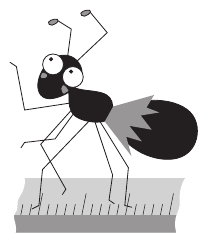
\includegraphics[scale=1]{pics/alice2}
\label{pic:alice2}
\caption{Элис прощается.}
\end{figure}
